\chapter{Introduction}
\label{chapter_1}

%% The following annotation is customary for chapter which have already been
%% published as a paper.
\blfootnote{Parts of this chapter have been published in Annalen der Physik \textbf{324}, 289 (1906) \cite{Einstein1906}.}

%% It is only necessary to list the authors if multiple people contributed
%% significantly to the chapter.
\authors{Albert {\titleshape Einstein}}

%% The '0pt' option ensures that no extra vertical space follows this epigraph,
%% since there is another epigraph after it.
\epigraph[0pt]{
    Nature and nature's laws lay hid in the night; \\
    God said `Let Newton be!' and all was light.
}{Alexander Pope}

\epigraph{
    It did not last: the devil shouting `Ho. \\
    Let Einstein be!' restore the status quo.
}{Sir John Collings Squire}

\begin{abstract}
Lorem ipsum dolor sit amet, consectetur adipisicing elit, sed do eiusmod tempor incididunt ut labore et dolore magna aliqua. Ut enim ad minim veniam, quis nostrud exercitation ullamco laboris nisi ut aliquip ex ea commodo consequat. Duis aute irure dolor in reprehenderit in voluptate velit esse cillum dolore eu fugiat nulla pariatur. Excepteur sint occaecat cupidatat non proident, sunt in culpa qui officia deserunt mollit anim id est laborum.
\end{abstract}

%% Start the actual chapter on a new page.
\newpage

\noindent This document is intended to be both an example of the TU Delft dissertation template for \LaTeX, as well as a short introduction to its use. It is not intended to be a general introduction to \LaTeX{} itself,\footnote{We recommend \url{http://en.wikibooks.org/wiki/LaTeX} as a reference and a starting point for new users.} and we will assume the reader to be familiar with the basics of creating and compiling documents.

Instructions on how to use this template under Windows and Linux, and which \LaTeX{} packages are required, can be found in \texttt{README.txt}.

\section{Document Structure}

\dropcap{S}{ince} a dissertation is a substantial document, it is convenient to break it up into smaller pieces. In this template we therefore give every chapter its own file. The chapters (and appendices) are gathered together in \texttt{dissertation.tex}, which is the master file describing the overall structure of the document. \texttt{dissertation.tex} starts with the line

%% We need an empty line before the quote environment to work around a bug in
%% the lettrine package, from which the drop command is derived.
\begin{quote}
\texttt{\textbackslash documentclass\{dissertation\}}
\end{quote}
which loads the dissertation template. The template is based on the \LaTeX{} \texttt{book} document class and stored in \texttt{dissertation.cls}. The document class accepts several comma-separated options. By default, hyperlinks are shown in cyan, which is convenient when reading the dissertation on a computer, but can be expensive when printing. They can be turned black with the \texttt{print} option. This will also turn the headers dark gray instead of cyan. Moreover, it will add a 3~mm bleed around the page including crop marks. This will help the printer with the thumb indices, since they run right up to the page borders. Finally, the \texttt{nativefonts} option can be used to override the automatic font selection (see below).

A dissertation is a big document, which makes it easy to miss warnings about the layout in the \LaTeX{} output. In order to locate problem areas, add the \texttt{draft} option to the \texttt{\textbackslash documentclass} line. This will display a vertical bar in the margins next to the paragraphs that require attention.

The contents of the dissertation are included between the \texttt{\textbackslash begin\{document\}} and \texttt{\textbackslash end\{document\}} commands, and split into three parts by
\begin{enumerate}
\item\texttt{\textbackslash frontmatter}, which uses Roman numerals for the page numbers and is used for the title page and the table of contents;
\item\texttt{\textbackslash mainmatter}, which uses Arabic numerals for the page numbers and is the style for the chapters;
\item\texttt{\textbackslash appendix}, which uses letters for the chapter numbers, starting with `A'.
\end{enumerate}
The title page is defined in \texttt{title.tex} in the \texttt{title} folder and included verbatim with \texttt{\textbackslash include\{title/title\}},\footnote{Note that it is not necessary to specify the file extension.} (see below). Additionally, it is possible to include a preface, containing, for example, the acknowledgements. An example can be found in \texttt{preface.tex}. The table of contents is generated automatically with the \texttt{\textbackslash tableofcontents} command. Chapters are included after \texttt{\textbackslash mainmatter} and appendices after \texttt{\textbackslash appendix}. For example, \texttt{\textbackslash include\{chapter-1/chapter-1\}} includes \texttt{chapter-1.tex}, which contains this introduction.

\section{Title Page}

\dropcap{T}{he} title pages are defined in \texttt{title/title.tex}, which you will have to modify according to your needs. Note that these pages are subject to the requirements of the \emph{promotieregelement} and cannot be changed at will. Apart from the names and dates, most of the Dutch text is dictated literally.

Since the thesis title and name of the author appear several times throughout the document (on the title page, but also in, \emph{e.g.}, the preface and cv), special commands are provided so they only have to be specified once. The title (and optional subtitle) can be specified with

\begin{quote}
\texttt{\textbackslash title[Optional subtitle]\{Title\}}
\end{quote}
The name of the author is specified with
\begin{quote}
\texttt{\textbackslash author\{First name\}\{Last name\}}
\end{quote}
Note that the first and last name are separate arguments, since they may be printed in different font shapes. The \texttt{\textbackslash title} and \texttt{\textbackslash author} commands also ensure that the title and author appear in the metadata of the final PDF.

See \texttt{title/title.tex} for detailed documentation on the comment and layout of the title pages. Logos of institutes that have contributed financially to the dissertation may be included on reverse side of the title page. A few example logos can be found in the \texttt{title/logos} folder.

\section{Chapters}

\dropcap{E}{ach} chapter has its own file. For example, the \LaTeX{} source of this chapter can be found in \texttt{chapter-1.tex}. A chapter starts with the command

\begin{quote}
\texttt{\textbackslash chapter\{Chapter title\}}
\end{quote}
This starts a new page, prints the chapter number and title and adds a link in the table of contents. If the title is very long, it may be desirable to use a shorter version in the page headers and the table of contents. This can be achieved by specifying the short title in brackets:

\begin{quote}
\texttt{\textbackslash chapter[Short title]\{Very long title with many words which could not possibly fit on one line\}}
\end{quote}
Unnumbered chapters, such as the preface, can be created with \texttt{\textbackslash chapter*\{Chapter title\}}. Such a chapter will not show up in the table of contents or in the page header. To create a table of contents entry anyway, add
\begin{quote}
    \texttt{\textbackslash addcontentsline\{toc\}\{chapter\}\{Chapter title\}}
\end{quote}
after the \texttt{\textbackslash chapter} command. To print the chapter title in the page header, add
\begin{quote}
    \texttt{\textbackslash setheader\{Chapter title\}}
\end{quote}

If (parts of) the chapter have already been published elsewhere, it is customary to add a reference. This can be done with the special unnumbered footnote command \texttt{\textbackslash blfootnote}. For example,

\begin{quote}
\texttt{\textbackslash blfootnote\{Parts of this chapter have been published in Annalen der Physik \textbackslash textbf\{324\}, 289 (1906) \textbackslash cite \{Einstein1906\}.\}}
\end{quote}
generates the footnote at the beginning of this chapter. Because this footnote is unnumbered, the \texttt{hyperref} package may throw a warning, which safely be ignored.

If multiple people have contributed significantly to this chapter, they can be lister with the \texttt{\textbackslash authors} command. This can be followed by a quotation using \texttt{\textbackslash epigraph} as shown above. Finally, it is customary for a dissertation to include an abstract for every chapter (except perhaps the introduction). This can be accomplished with the \texttt{abstract} environment. The abstract should be followed by \texttt{\textbackslash newpage} to start the chapter text on a new page.

In a dissertation, each chapter has its own list of references. These can be generated with the special command \texttt{\textbackslash references\{dissertation\}} from \texttt{dissertation.bib} at the end of the chapter. Note that this means that you need to run a command like \texttt{bibtex chapter-1/chapter-1} for each chapter. The bibliography style is specified in \texttt{dissertation.bst}, which is a modified version of \texttt{apsrev4-1.bst} (from REVTeX) designed to also display the titles of referenced articles. The template will automatically generate clickable hyperlinks if a URL or DOI (digital object identifier) is present for the reference. Although it is possible to manage the bibliography by hand, we recommend using EndNote (available from Blackboard) or JabRef (available from \url{http://jabref.sourceforge.net/}).

Chapters are subdivided into sections, subsections, subsubsections, and, optionally, paragraphs and subparagraphs. All can have a title, but only sections and subsections are numbered. As with chapters, the numbering can be turned off by using \texttt{\textbackslash section*\{\ldots\}} instead of \texttt{\textbackslash section\{\ldots\}}, and similarly for the subsection.
\section{\textbackslash section\{\ldots\}}
\subsection{\textbackslash subsection\{\ldots\}}
\subsubsection{\textbackslash subsubsection\{\ldots\}}
\paragraph{\textbackslash paragraph\{\ldots\}}
Lorem ipsum dolor sit amet, consectetur adipisicing elit, sed do eiusmod tempor incididunt ut labore et dolore magna aliqua. Ut enim ad minim veniam, quis nostrud exercitation ullamco laboris nisi ut aliquip ex ea commodo consequat. Duis aute irure dolor in reprehenderit in voluptate velit esse cillum dolore eu fugiat nulla pariatur. Excepteur sint occaecat cupidatat non proident, sunt in culpa qui officia deserunt mollit anim id est laborum.

\section{Fonts and Colors}

\dropcap{T}{he} fonts used by this template depend on which version of \LaTeX{} you use. Regular \LaTeX, \emph{i.e.}, if you compile your document with with \texttt{latex}, \texttt{pslatex} or \texttt{pdflatex}, 
will use KP-Fonts, with Latin Modern as a fallback.
% will use Utopia for text, Fourier for math and Latin Modern for sans-serif and monospaced text. 
However, if you want to adhere to the TU Delft house style, you will need to use \XeLaTeX, as it supports TrueType and OpenType fonts. Compiling with \texttt{xelatex} will use Bookman Old Style for titles, Tahoma for text, Courier New for monospace and Cambria for math. If you want to use \XeLaTeX, but do not want to use the TU Delft house style fonts, you can add the \texttt{nativefonts} option to the document class.

This template supports the use of drop caps, a large colored initial at the beginning of a chapter or section, via the \texttt{\textbackslash dropcap} command:

\begin{quote}
\texttt{\textbackslash dropcap\{L\}\{orem\} ipsum\ldots}
\end{quote}
The first argument is the capital that will be printed on two lines (in the title color), and the second argument is the rest of the word. Depending on the font, the latter may be printed in small caps.

The original TU Delft template extensively used the corporate colors cyan, black and white. This adapted version has only black text by default. However, if you are wish to use the TU Delft colors, you can access them through commands such as \texttt{\textbackslash color\{{\color{tudelft-cyan}tudelft-cyan}\}}, \texttt{\textbackslash color\{{\color{tudelft-black}tudelft-black}\}} (which differs slightly from the default \texttt{black}) and \texttt{\textbackslash color\{tudelft-white\}}. Apart from these three, the house style defines the basic colors
\begin{itemize}
%% Reduce the separation between the items, since this is just a list of words.
\itemsep 0pt
\parskip 0pt
\item\texttt{\color{tudelft-sea-green}tudelft-sea-green},
\item\texttt{\color{tudelft-green}tudelft-green},
\item\texttt{\color{tudelft-dark-blue}tudelft-dark-blue},
\item\texttt{\color{tudelft-purple}tudelft-purple},
\item\texttt{\color{tudelft-turquoise}tudelft-turquoise} and
\item\texttt{\color{tudelft-sky-blue}tudelft-sky-blue},
\end{itemize}
as well as the accent colors
\begin{itemize}
\itemsep 0pt
\parskip 0pt
\item\texttt{\color{tudelft-lavendel}tudelft-lavendel},
\item\texttt{\color{tudelft-orange}tudelft-orange},
\item\texttt{\color{tudelft-warm-purple}tudelft-warm-purple},
\item\texttt{\color{tudelft-fuchsia}tudelft-fuchsia},
\item\texttt{\color{tudelft-bright-green}tudelft-bright-green} and
\item\texttt{\color{tudelft-yellow}tudelft-yellow}.
\end{itemize}

% Break up figure captions into two pages
\begin{figure}
\centering
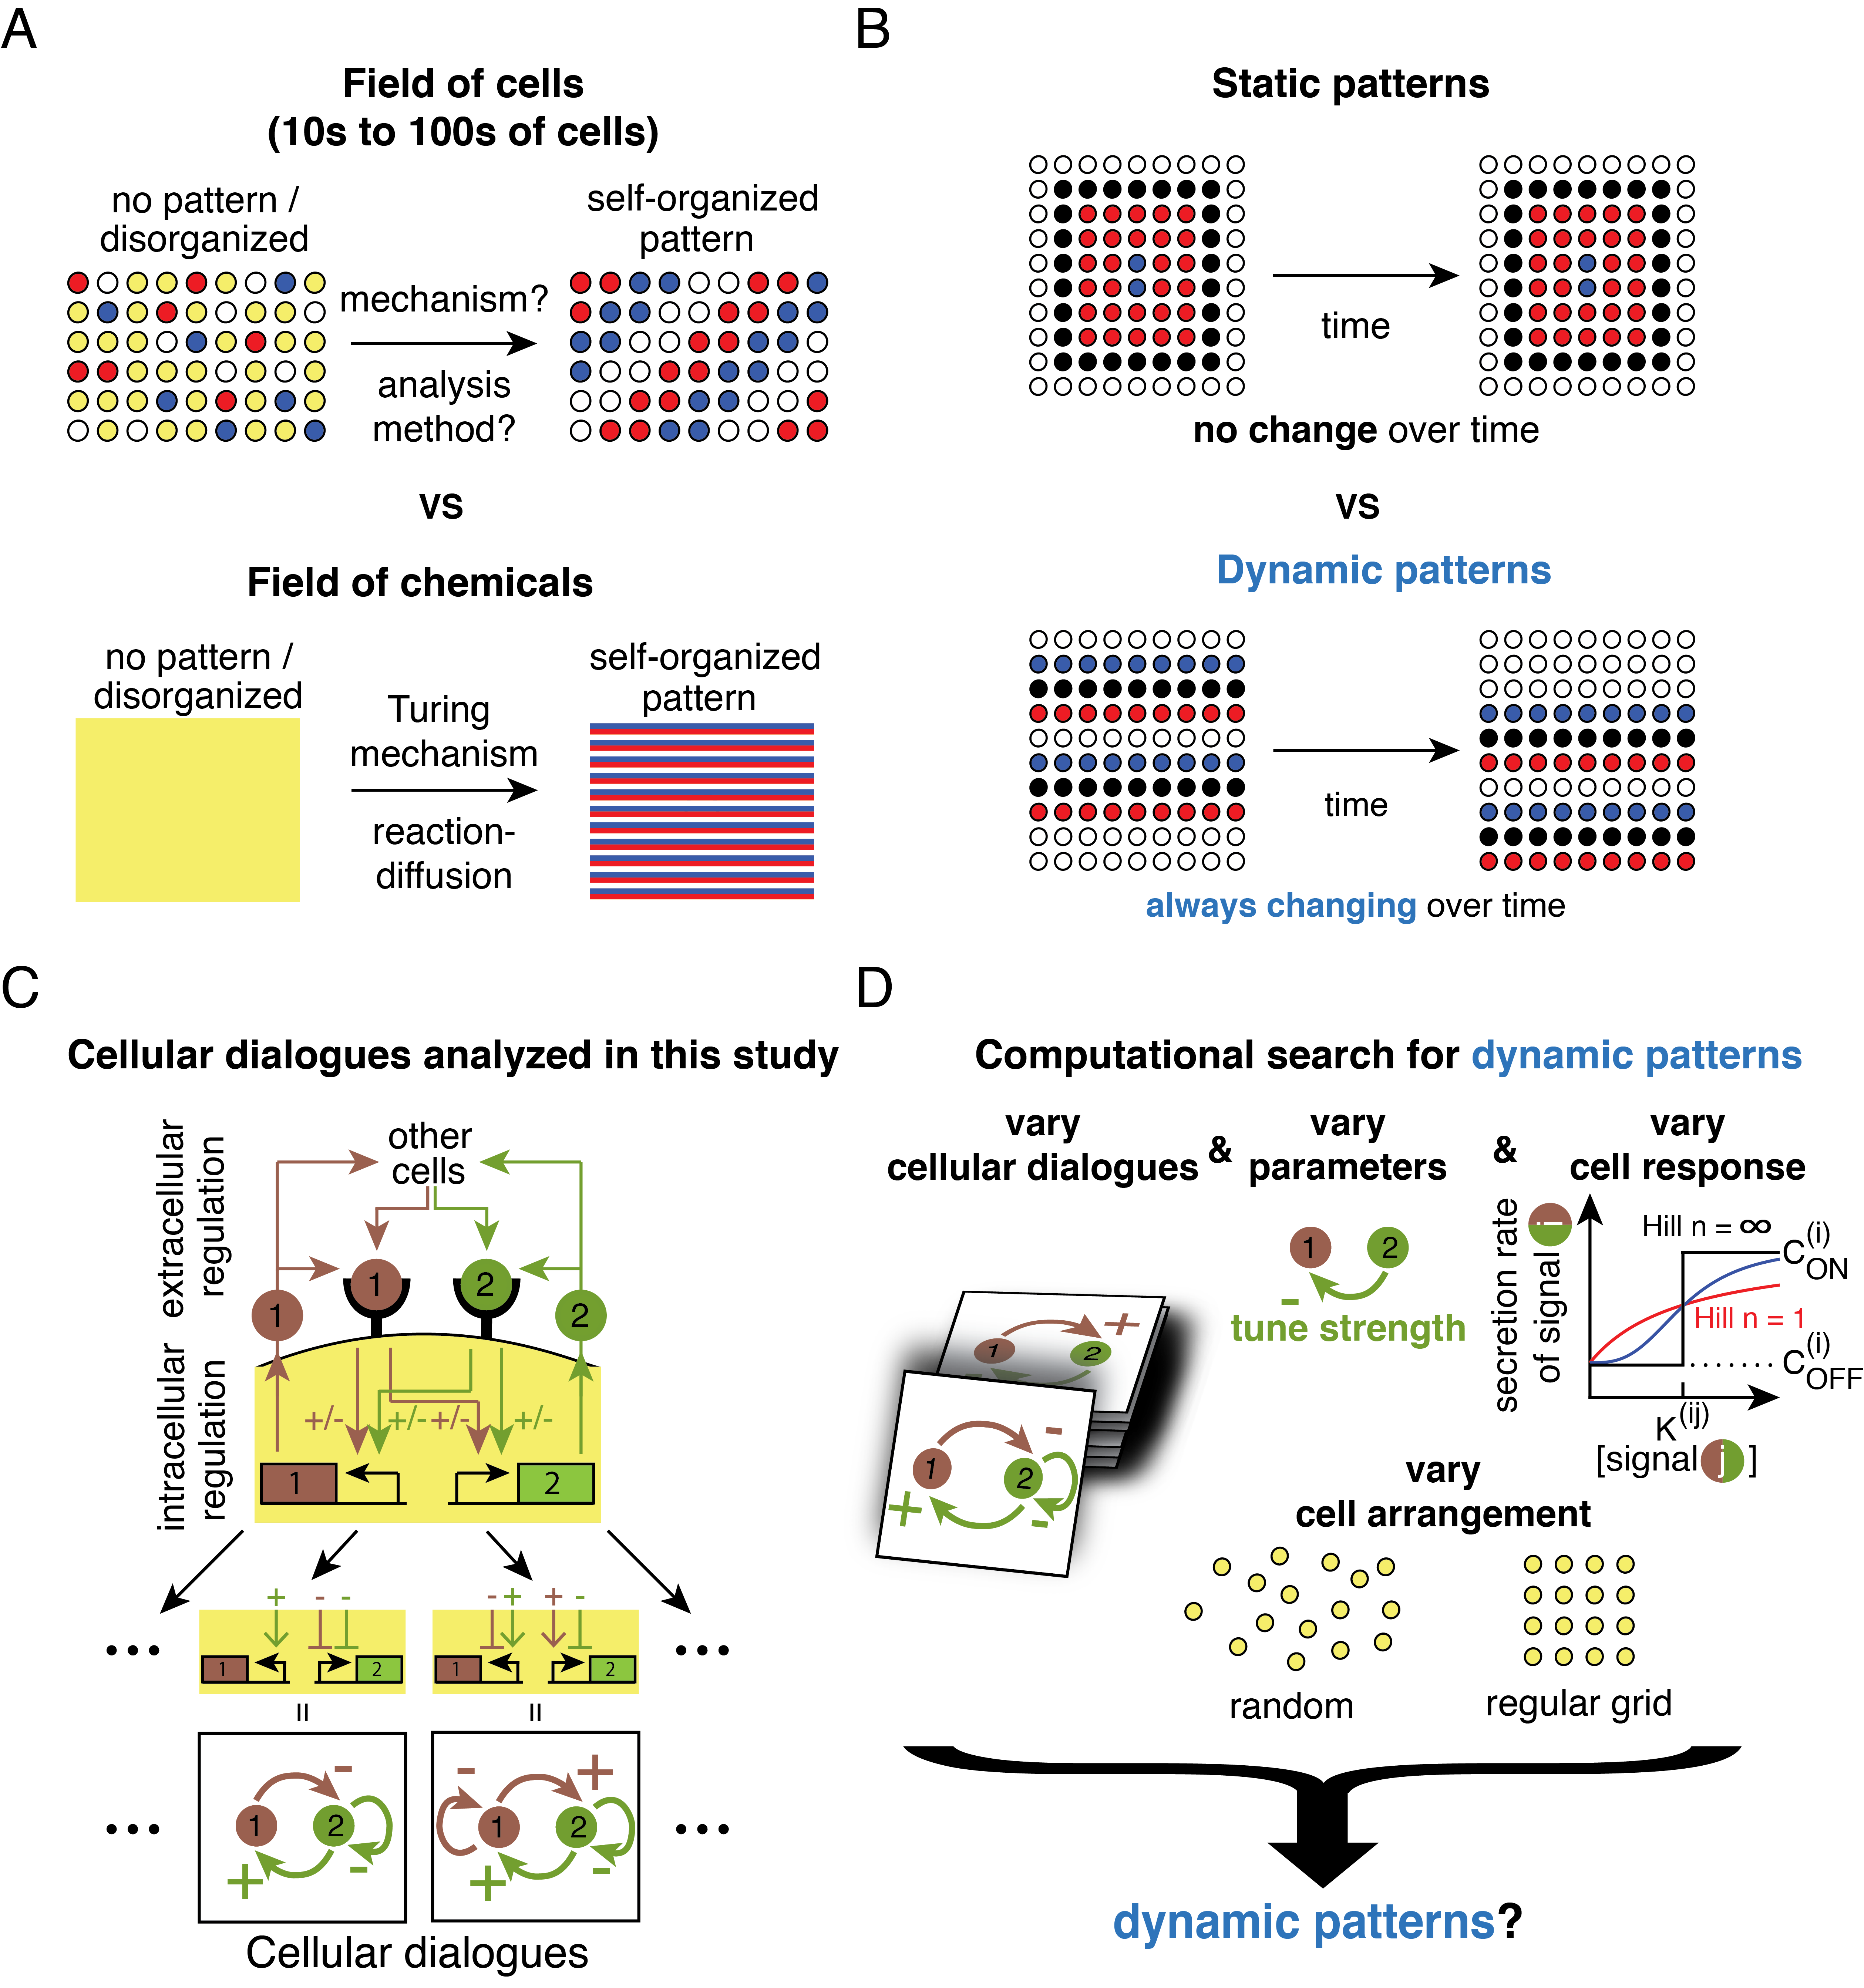
\includegraphics[width=\textwidth]{./chapter-1/figures/Fig1_Dang_cell-circuits_191215.png}
\caption[A random figure from another thesis]{
\textbf{A random figure from another thesis.}
\textbf{Computationally screening cellular dialogues to find ones that enable dynamic patterns to form.} 
\textbf{(A)} Pattern formation by cells versus chemicals. (Top) Mechanisms by which an initially disordered field of a mesoscopic number of cells ($\mathrm{\sim}$hundreds to thousands) (left panel) become more ordered through cell-cell communication (right panel) remain poorly understood, as is the method to analyze this complex self-organization dynamics. (Bottom) A field of chemicals or a continuum of cells (large number of tightly packed cells) initially having no pattern (left) can form a pattern (right) without pre-existing morphogens. This is usually modelled by reaction-diffusion equations and can be understood through the Turing mechanism. 
\textbf{(B)} Static versus dynamic patterns. (Top) Static patterns do not change over time. (Bottom) In dynamic patterns, a structure changes over time without ever stopping (e.g., shown here is a traveling wave). 
(\emph{Caption continued on next page.})
}
\end{figure}

\begin{figure}
\captionsetup{labelformat=adja-page}
\ContinuedFloat
\caption[]{
\textbf{For large pictures, break up caption into multiple pages with fltpage package.}
\textbf{(C)} Schematic of cellular dialogues. Brown (molecule 1) and green (molecule 2) circles are ligands that bind to their cognate receptors on the cell membrane. Ligand-bound receptors trigger intracellular signal transductions that either positively or negatively regulate the production and secretion of molecules 1 and 2 (molecule 1 can self-promote or self-repress its own secretion while also regulating the secretion of molecule 2, and vice versa). Bottom row shows graphic representation of cellular dialogues. 
\textbf{(D)} Elements that we varied in simulations: cellular dialogues of all possible topologies, the values of the parameters for each cellular dialogue, and spatial arrangement of cells. Our study first begins with an infinite Hill coefficient (i.e., digital response to each of the two signaling molecules) and a regular lattice. After reporting the outcomes of these simulations, we report the result of relaxing these two constraints and well as other elements not depicted.
}
\label{fig:ChIV:1}
\end{figure}

